% author: Tomas Trnka
% mail: tomas@trnkatomas.eu
% date: 2013-07-04

\documentclass[a4paper,10pt]{article}
%\usepackage[czech]{babel}
%\usepackage[T1]{fontenc}
\usepackage[hmargin=2.2cm,vmargin=2.2cm]{geometry}
\usepackage[utf8x]{inputenc}
\usepackage{fancyhdr}
\usepackage{fancyvrb}
\usepackage{amsmath} 
\usepackage{float}
\usepackage{enumerate}
\usepackage{tikz}
\usepackage{hyperref}
\pagestyle{fancy}
\headheight 15pt
\lhead{Crpyto, Fall 2014}
\rhead{Tomas Trnka}
\newcommand{\set}[1]{\ensuremath{\left\lbrace #1 \right\rbrace}}
\newcommand{\role}[1]{\ensuremath{\left\langle #1 \right\rangle}}
\newcommand{\cara}{\begin{center}\rule{140mm}{.2mm}\end{center}}
\newcommand{\mI}{\ensuremath{^\mathcal{I}}}
\newcommand{\Tbox}[1]{\ensuremath{\mathcal{T}}-Box#1}
\newcommand{\Abox}[1]{\ensuremath{\mathcal{A}}-Box#1}
\newcommand{\mC}[1]{\ensuremath{\mathcal{#1}}}
\newcommand{\Tc}{\ensuremath{\mathcal{T}_c}}
\newcommand{\qb}[1]{\ensuremath{\vert{#1}\rangle}}
\newcommand{\mc}[1]{\ensuremath{\mathcal{#1}}}
\begin{document}
\section*{Perfect Security and Information Theory}
\subsection*{Security}
\begin{itemize}
\item \textbf{computational security}\\ it concerns only about computational effort that is required to break a cryptosystem, it means that solve such task one needs at least N operations that are not solvable by current machines in reasonable time. This measure does not guarantee against other attacks.
\item \textbf{provable security}\\
this measure is sort of comparison against well known problem where we know how difficult they are, it somewhat similar to polynomial reduction when we say that this task is at least as difficult as NP.
\item \textbf{unconditional security}
unconditional security is such a security that cannot be broken even with infinite computational resources
\end{itemize}
\subsection*{Probability}
Unconditional security can be studied from the point of view of probability.
Discrete random variable is
$$
0 \leq Pr[X=x], \sum_{x \in X} Pr[X=x] = 1
$$

Multiple random variable, suppose there exist $X$ and $Y$ random variables then we can define \textit{joint} and \textit{conditional} probability. They are denotes as $P[X=x,Y=y],Pr[X=x|y]$ respectively.

Joint probability of conditional probability is 
$$
Pr[x,y] = Pr[x|y]Pr[y] = Pr[y|x]Pr[x]
$$
and the result of these two equations is Bayes' theorem
$$
Pr[x|y] = \frac{Pr[x]Pr[y|x]}{Pr[y]}
$$
They are independent iff $Pr[x|y]=P[x]$
\subsection*{Perfect secrecy}
\textbf{Definition} A cryptosystem has \textit{perfect secrecy} if Pr[x|y] = Pr[x] for all $x \in \mathcal{P}, y \in \mathcal{C}$.

\noindent
\textbf{Theorem} Suppose $(\mc{P},\mc{C},\mc{K},\mc{E},\mc{D})$ is a cryptosystem where $|\mc{K}| = |\mc{C}| = |\mc{P}|$. Then the cryptosystem provides perfect secrecy iff every key is used with probability $\frac{1}{\mc{K}}$ and for every $x \in \mc{P}, y \in \mc{C}$, there is unique key K such that $e_K(x) = y$.

\subsubsection*{Application as one-time pad}
This system was believed as unbreakable but the proof comes just out of the Shannon theorem. The major drawback is that the key must be as long as the message and moreover that the key can be used only once. 

\subsection*{Entropy}
So far we looked at the situations where the key is used only once, now what happened when we use the same key multiple times?

Entropy can be interpreted as a measure of uncertainty or information, it is a function of probability distribution.

\noindent
\textbf{Definition}
Suppose X is a discrete random variable which takes on values from a finite set X. Then, the \textit{entropy} of the random variable X is defined to be the quantity
$$
H(X) = -\sum_{x\in X} \Pr[x]\log_2\Pr[x].
$$
(Possibly draw a 2D diagram of entropy - it is clear what is meant by the amount of information and what the logarithm does to it)

\subsubsection*{Properties of entropy}
We have to define what does it mean that function is concave.
$$
f\left( \frac{x+y}{2} \right) \geq \frac{f(x)+f(y)}{2}
$$
Jensen's inequality, suppose that f is strictly concave on interval $ I $ and also that $\sum_{i=1}^n a_i = 1$, and $a_i \geq 0, 1 \leq i \leq < n$. Then
$$
\sum_{i=1}^n a_i f(x_i) \leq f \left( \sum_{i=1}^n a_i x_i \right)
$$
where $x_i \in I, 1\leq i \leq n$.

\noindent
\textbf{Theorem} Suppose X is a random variable having a probability distribution which takes on the values $p_1,p_2,...,p_n$, where $ p_i \ge 0,1 \leq i \leq n$. Then $H(X) \leq \log_2 n$, with equality iff $p_i = \frac{1}{n},1 \leq i \leq n$.

\noindent
\textbf{Theorem} $H(X,Y) \leq H(X) + H(Y)$, with equality iff X and Y are independent random variables.

\noindent
\textbf{Definition} Suppose X and Y are two random variables. THen for any fices value y of Y we get a (conditional) probability distribution on X; we denote the associated random variable by X|y:
$$
H(X|y) = -\sum_x \Pr[x|y]\log_2 \Pr[x|y]
$$
We define conditional entropy H(X|Y) to be weighted average of the entropies H(X|y) over all possible values $y$.
$$
H(X|Y) = -\sum_y\sum_x\Pr[y]\Pr[x|y]\log_2\Pr[x|y].
$$
The conditional entropy measures the average amount of information about X that is not revealed by Y.

\noindent
\textbf{Theorem} $H(X,Y) = H(Y) + H(X|Y)$

\noindent
\textbf{Corollary} $H(X|Y) \leq H(X)$, with equality iff X and Y are independent.


\section*{Spurious Keys and Unicity Distance}
Spurious key are such keys that we are left with after we have ruled out many keys that would provide incorrect decryption. We would like to bound the amount of spurious keys. We at first define the entropy for the whole \mc{C} per letter.\\
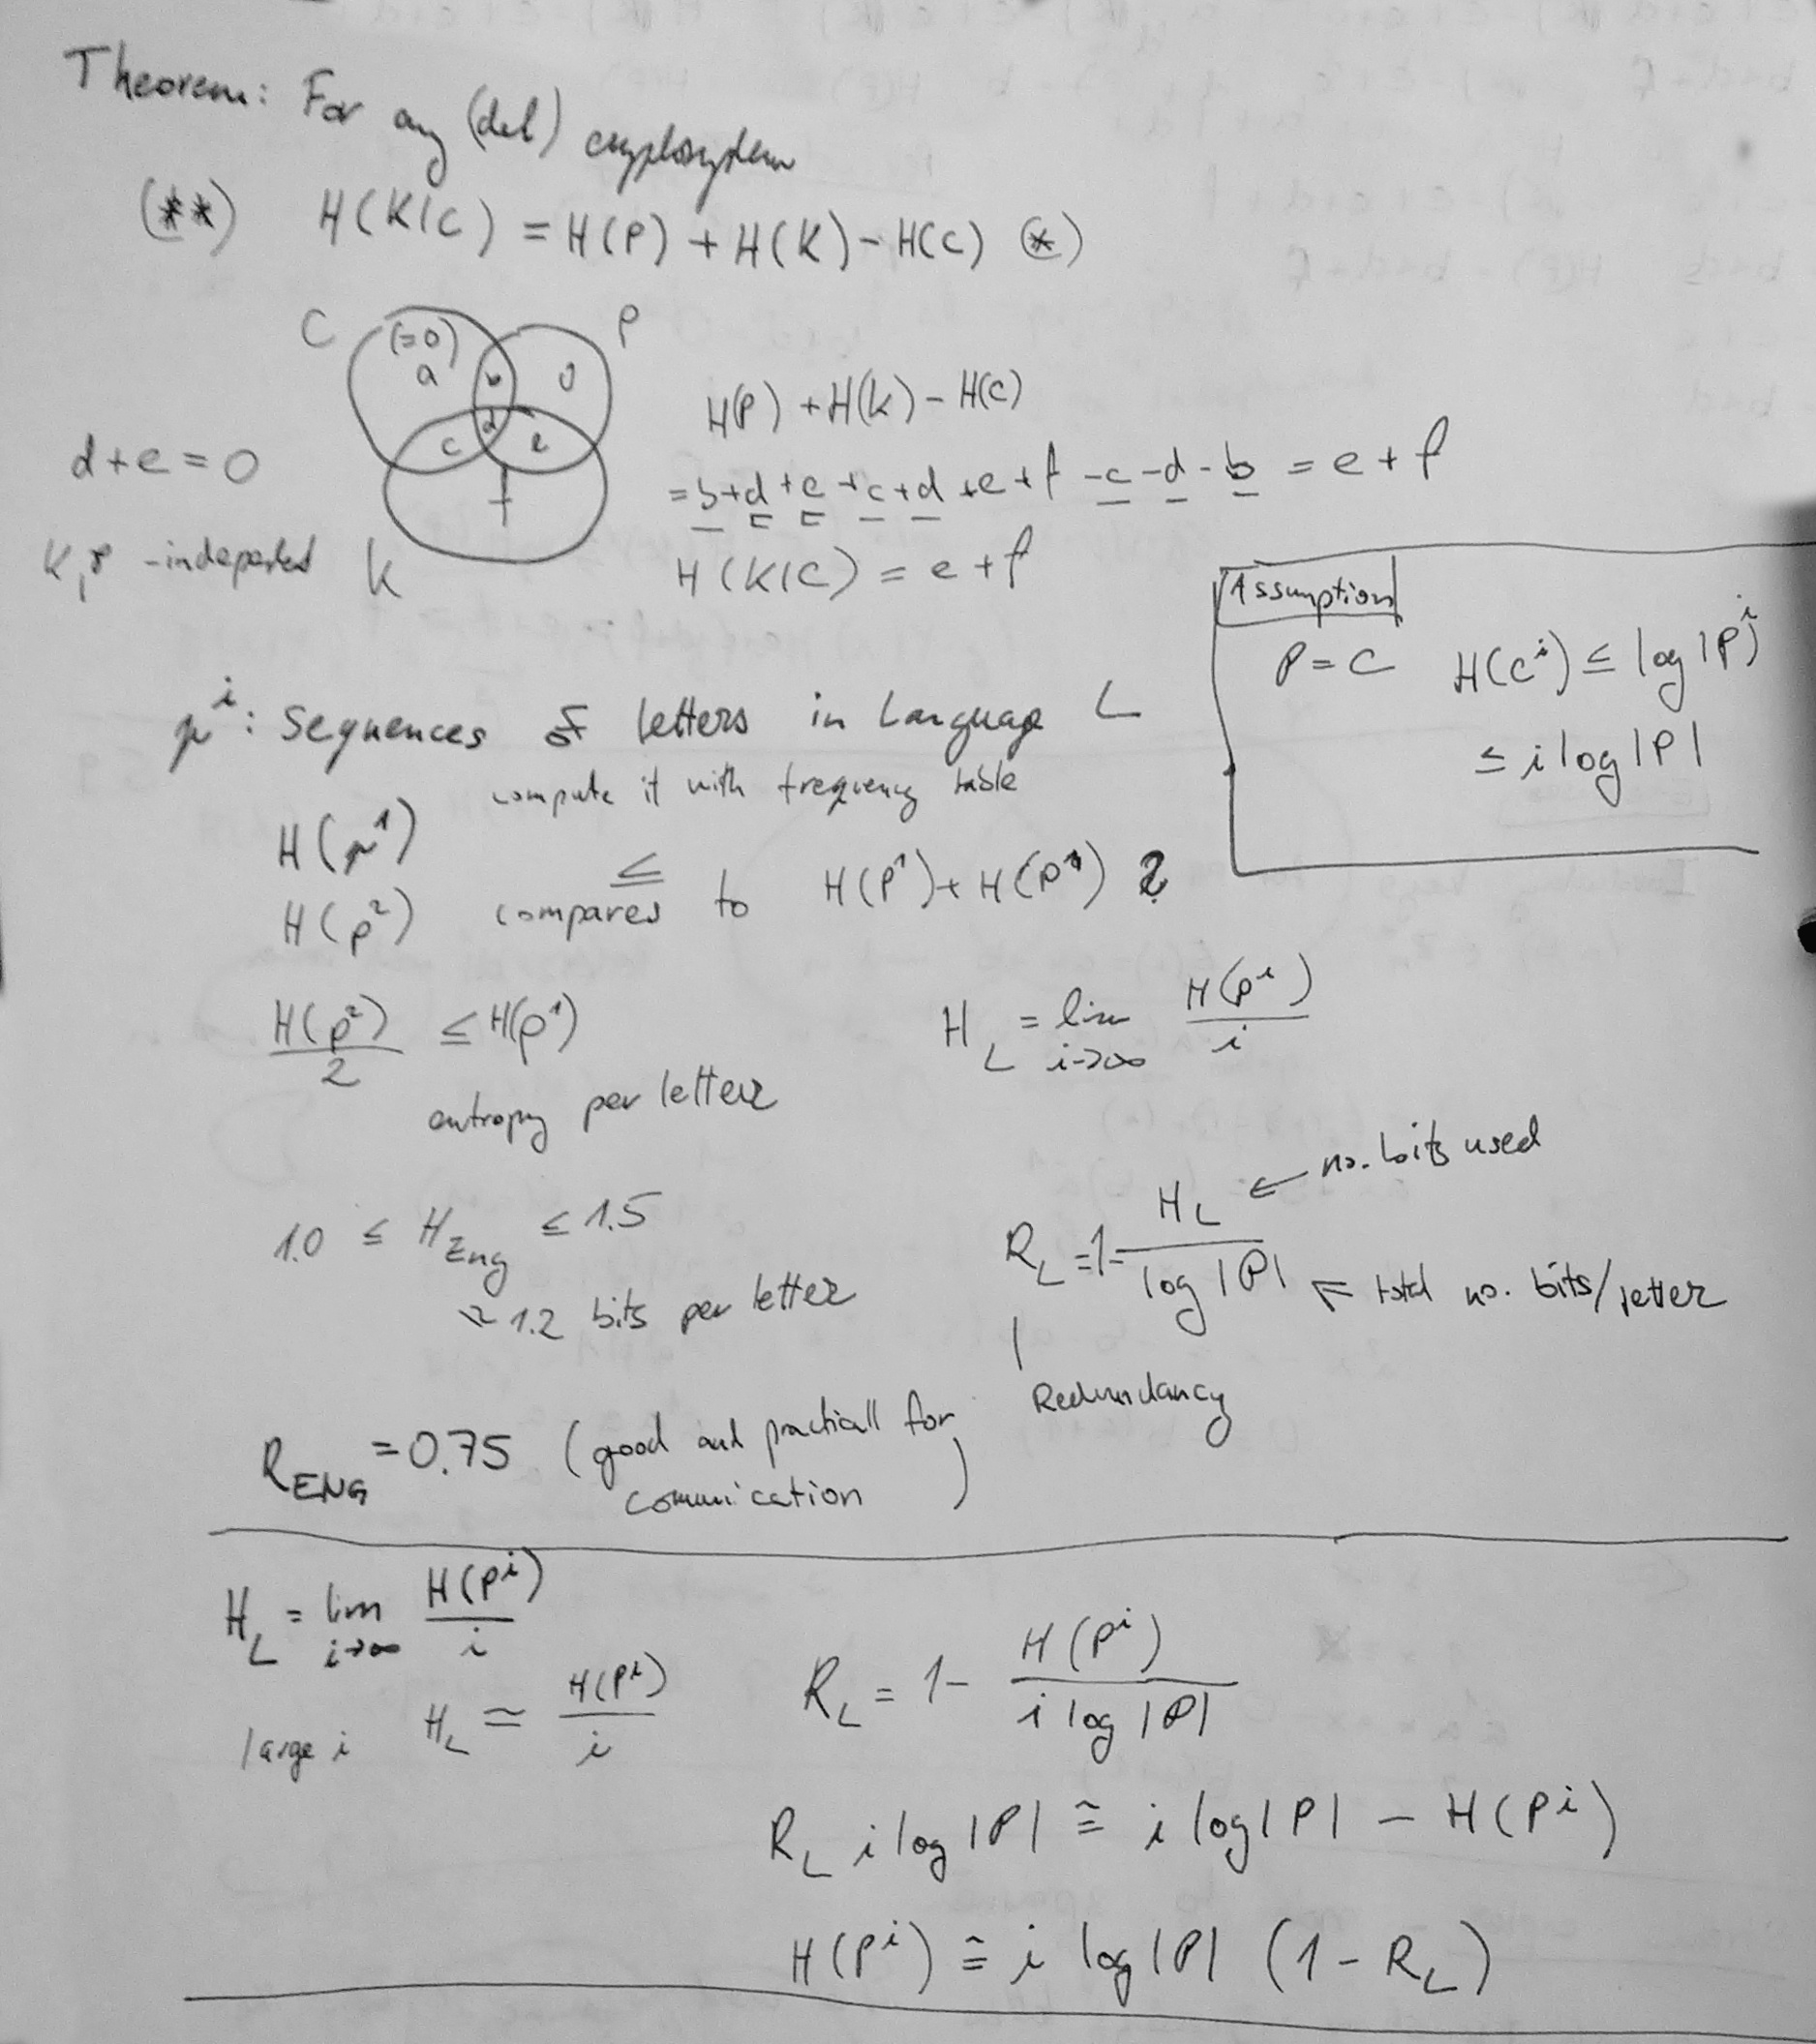
\includegraphics[width=\textwidth]{entropy.jpg}
The unicity distance of a cryptosystem is defined to be the value of $n$, denoted by $i$ at which the expected number of spurious keys become zero, i.e. the average amount of ciphertext required for an opponent to be abel to uniquely compute the key, given enough computing time.
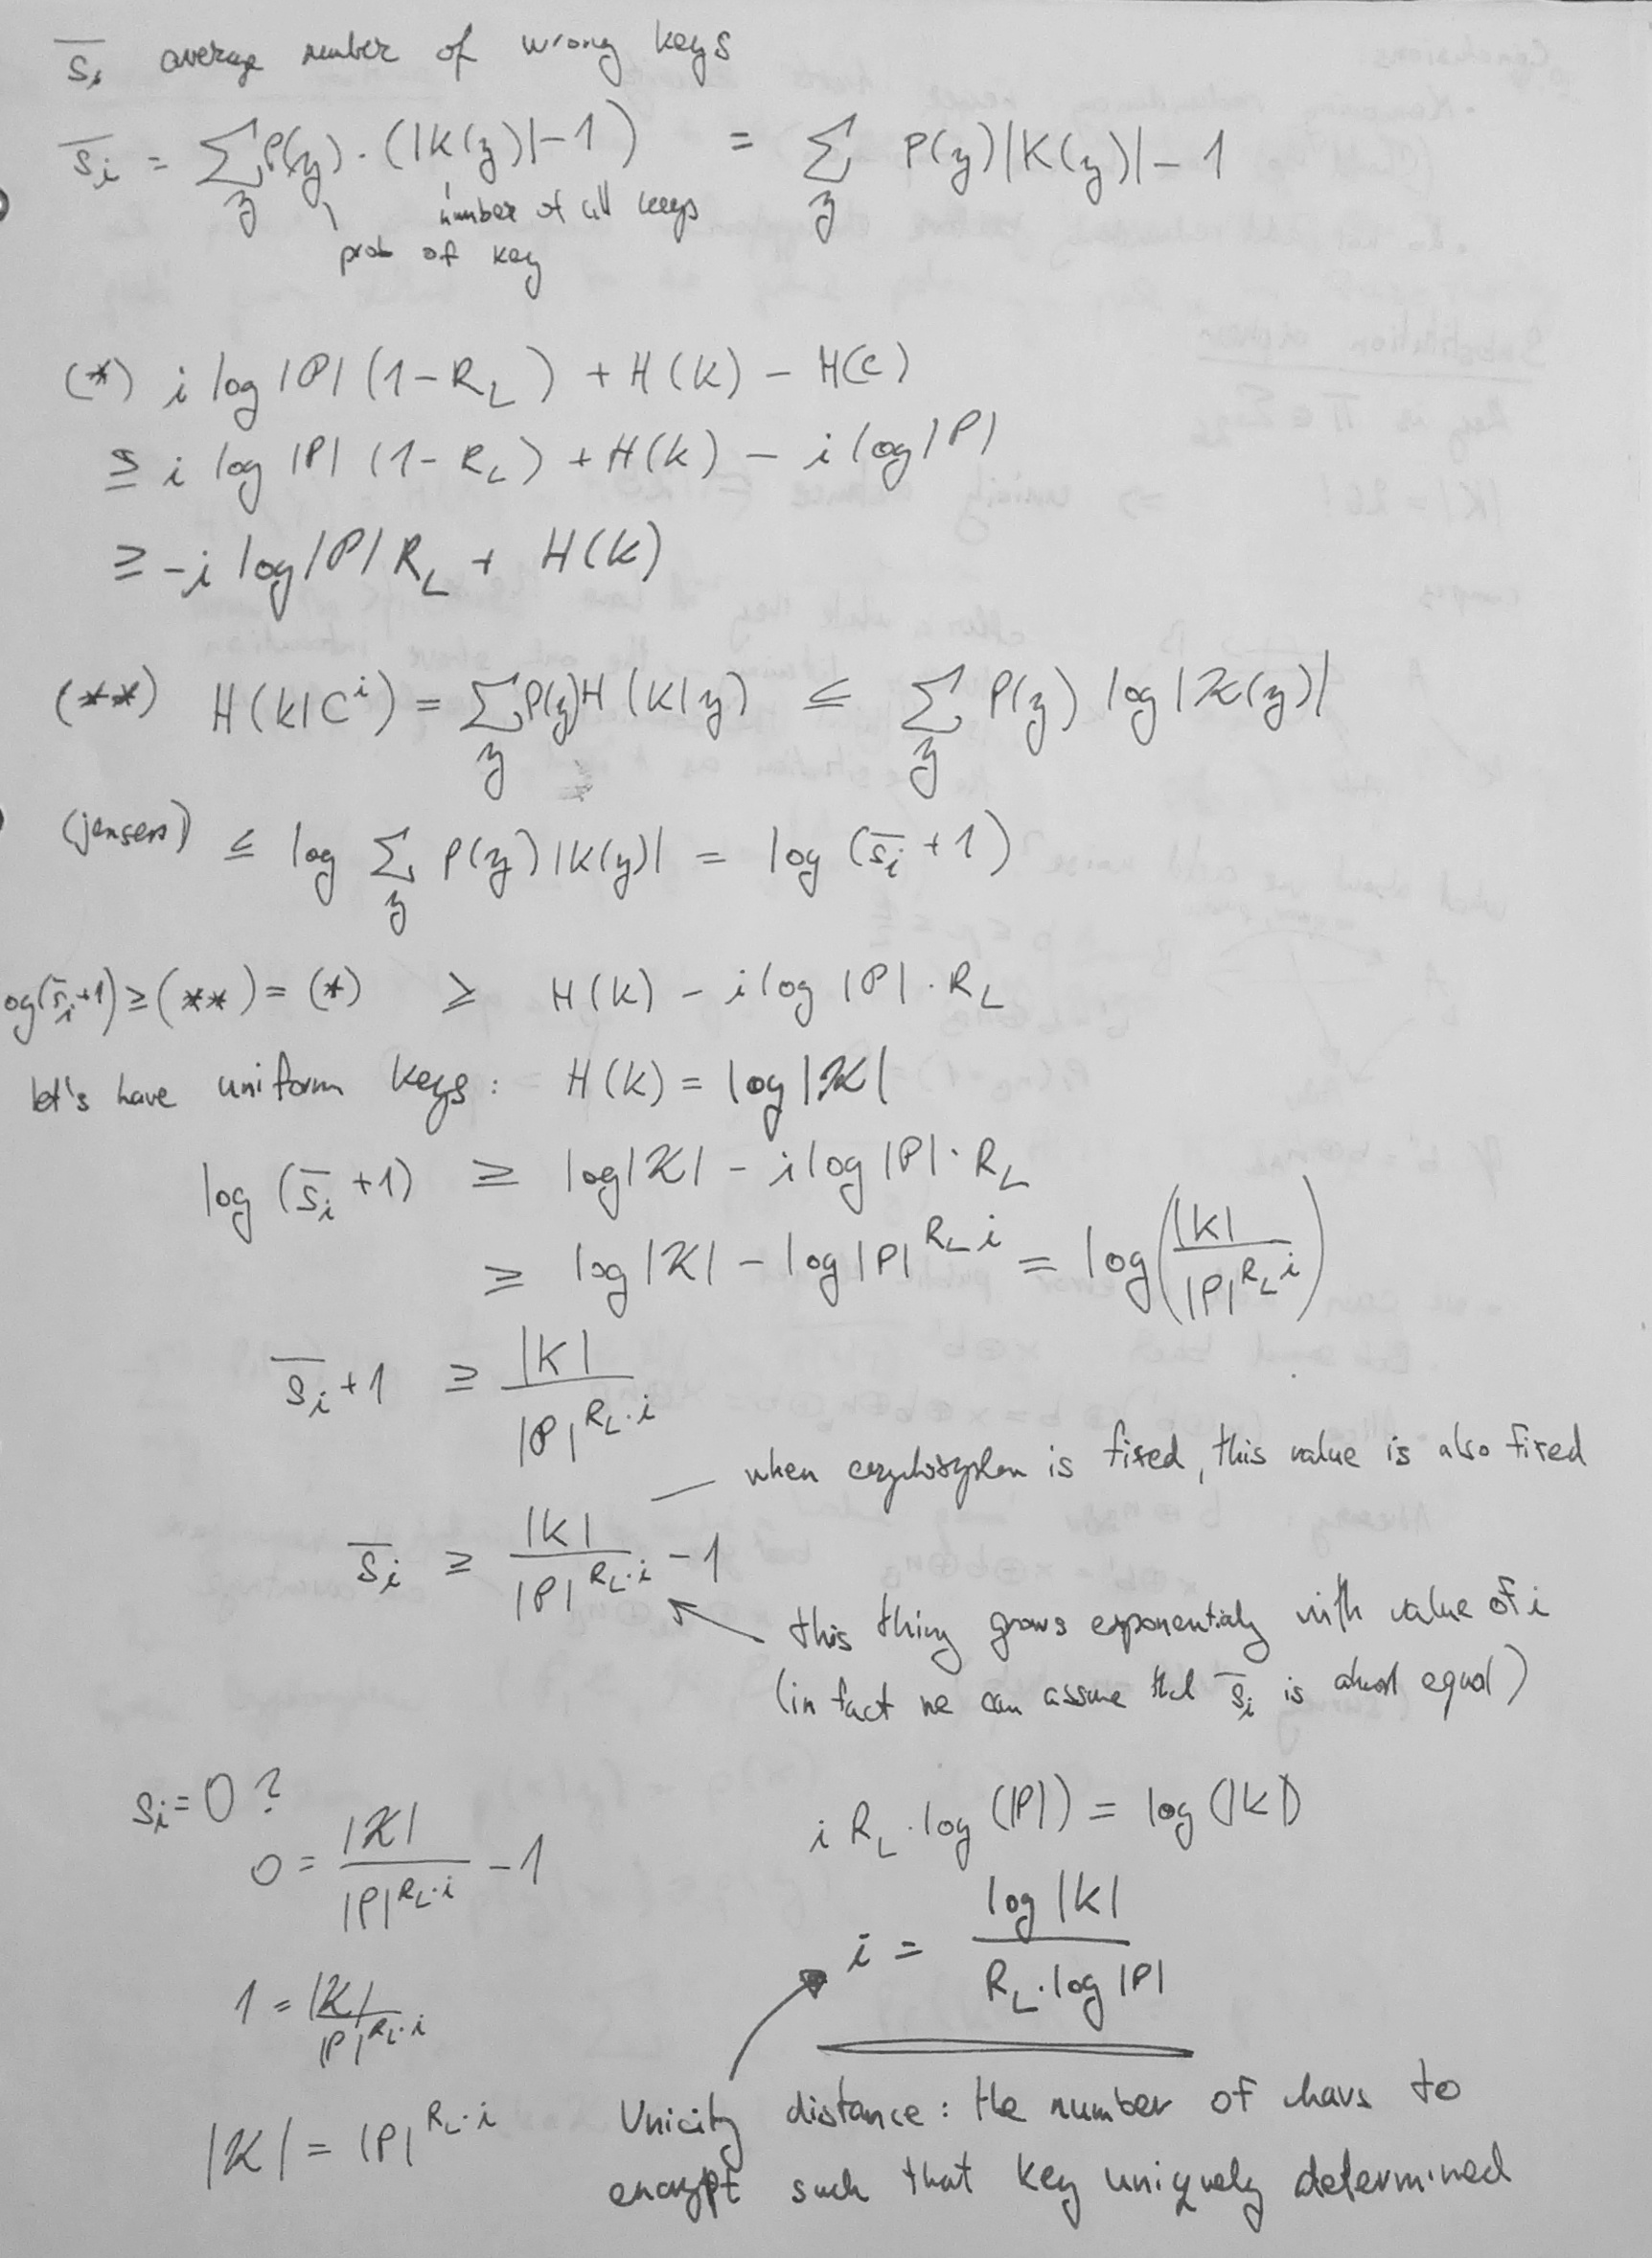
\includegraphics[width=\textwidth]{unicity_distance.jpg}
\subsection*{Product cryptosystems}
For some of them it just does not make sense, the most common used combination is shift and permutation. Some of these compound ciphers can be iterated to obtain better security. Examples useles (two affine ciphers, two shift ciphers).
\end{document}